\subsection{The quest to discover Majorana neutrinos}

The discovery of neutrino oscillations \cite{Super-Kamiokande:1998kpq,SNO:2001kpb,SNO:2002tuh} has established that neutrinos are massive
particles \cite{GonzalezGarcia:2002dz} and thus contradicted a fundamental postulate of the Standard Model (SM) of particle physics. In doing so, it has opened a window to the study of new phenomena, related with fundamental unknown properties of this particle. We do not know if neutrinos are Dirac fermions, which get their masses through the SM-prescribed coupling to the Higgs boson. Or if they are Majorana particles \cite{Majorana:1937}, a new type of matter in which particles and antiparticles can be described by the same quantum field (thus Majorana particles are said to be identical to their own antiparticles) and whose existence implies physics beyond the SM. In addition, given the interferometric nature of neutrino oscillation experiments, which can only measure squared mass differences, we know neither the absolute scale of neutrino masses, nor the type of the neutrino mass spectrum. Last but not least, we do not know if the CP symmetry is violated by neutrinos (as it is violated in the quark sector), and if that is the case, how large is the effect.

\indent

On the other hand, our current understanding of leptogenesis  \cite{Fukugita:1986hr, Fukugita:1998vn} requires
massive Majorana neutrinos and CP violation to produce the observed cosmic matter-antimatter asymmetry (see for example \cite{Sarkar:1998im} and references therein). Furthermore, Majorana neutrinos could provide an explanation of the smallness of the neutrino masses compared with that of the other leptons, through the so-called see-saw mechanism
\cite{GellMann:1980vs, Yanagida:1979as, Mohapatra:1979ia}. In conclusion, establishing if the neutrino is a Majorana particle is one of the most important long-standing questions in particle physics and cosmology.

\begin{figure}[h!]
\centering
%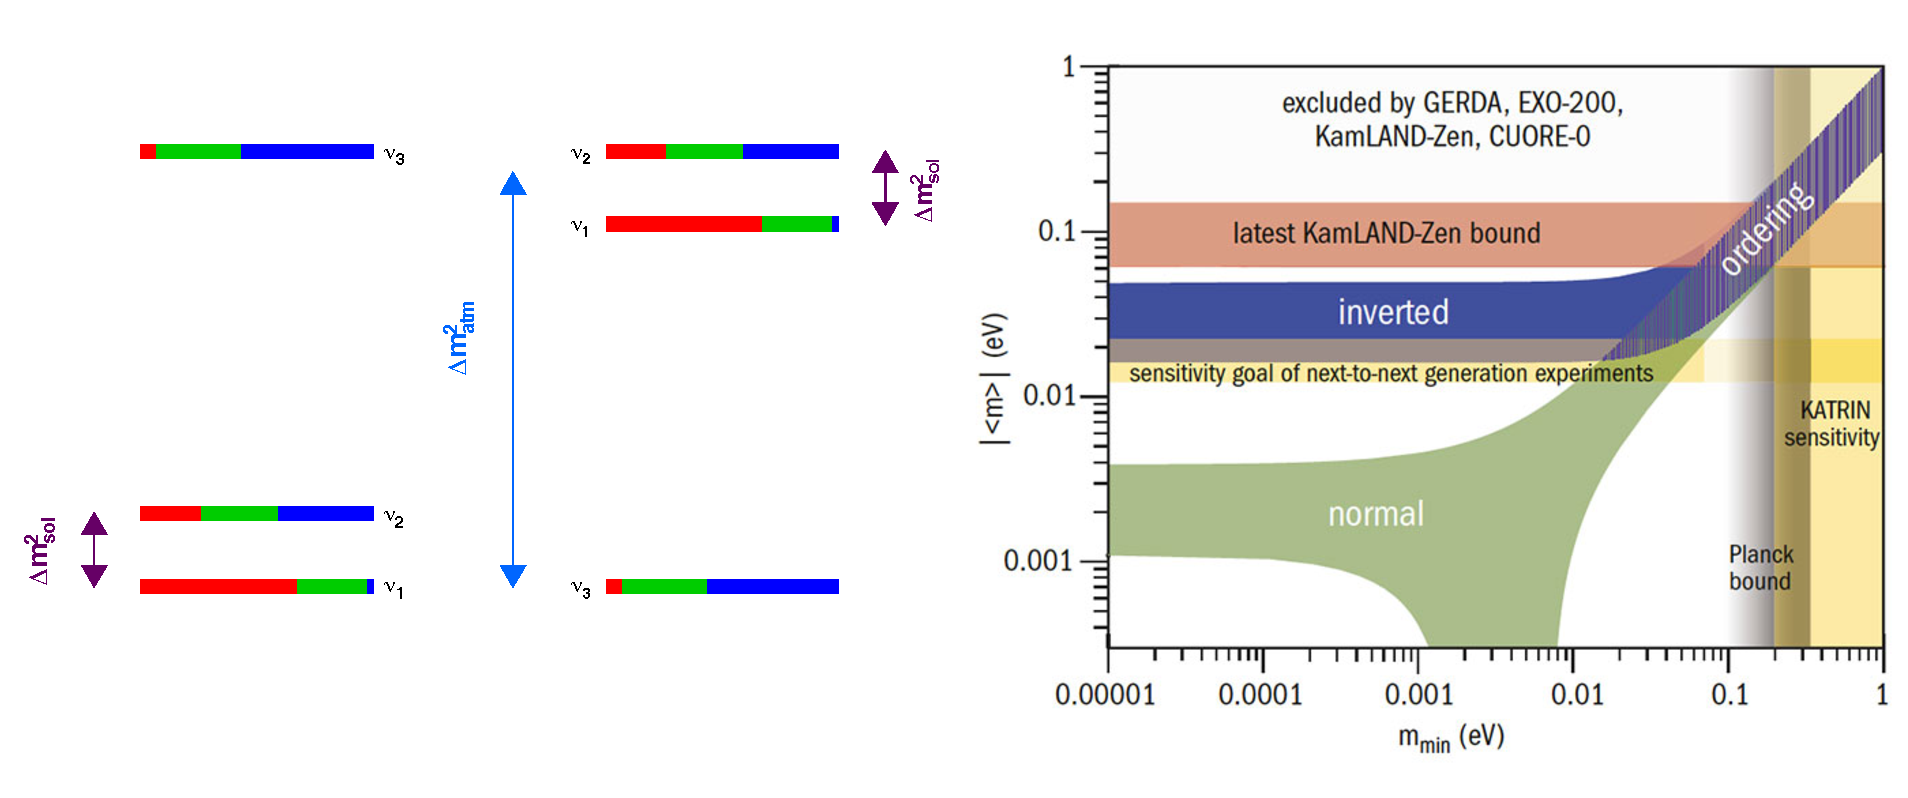
\includegraphics[width=\textwidth]{img/massesAndLandscape}
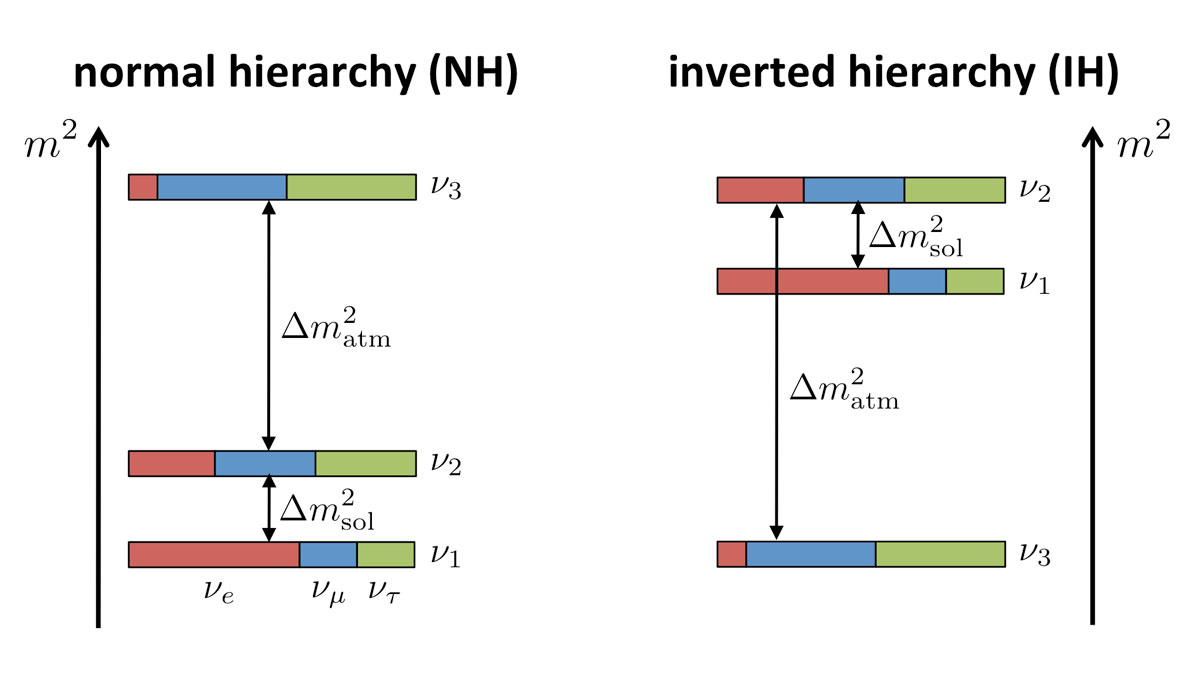
\includegraphics[width=0.49\textwidth]{img2/mass-hierarchy-jgu-mainz-web.jpg} \hfill
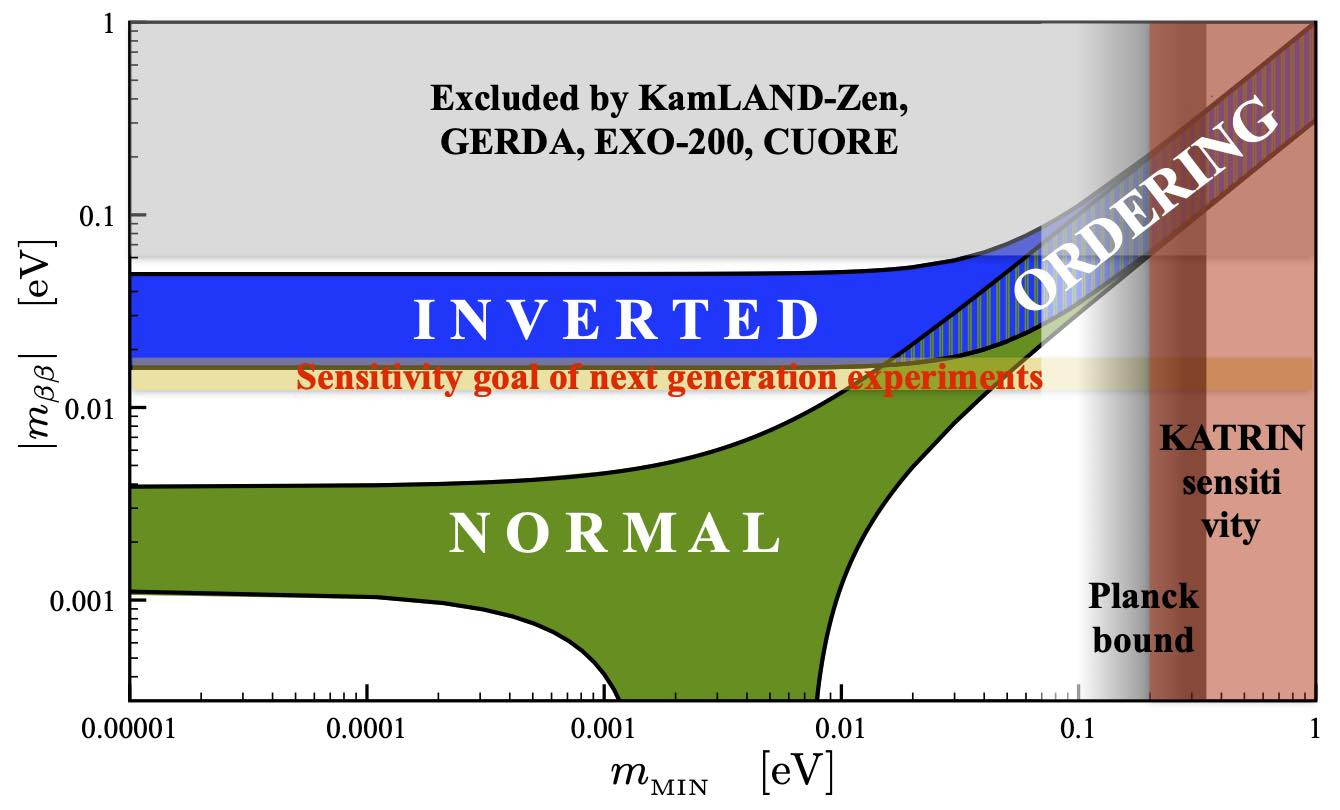
\includegraphics[width=0.49\textwidth]{img2/APPECbetabetameff.jpg}
%\vspace*{-7mm}
\caption{\small The left panel shows the NH (left) and IH (right) mass orderings. 
%The electron, muon and tau flavour content of each neutrino mass eigenstate is shown via the red, green and blue fractions, respectively.
The right panel \cite{Giuliani:2019uno} shows the effective neutrino Majorana mass, \mbb\, as a function of the lightest neutrino mass, $m_{\rm min}$.
The vertically-excluded region comes from cosmological bounds and direct mass measurements; the horizontally-excluded one from \bbonu\ constraints.} \label{fig:numass_ordering}
\end{figure}
%%%%%%%%%%

\indent

Neutrino oscillation experiments have measured two mass splittings. The so-called \emph{solar mass splitting}, $\Delta m^2_{ \rm sol}\equiv m^2_2-m^2_1\sim 7.4 \times
10^{-5}\ {\rm eV}^2$ and the
\emph{atmospheric mass splitting}, $|\Delta m^2_{\rm
atm}|\equiv |m^2_3-m^2_2|\simeq|m^2_3-m^2_1| \sim 2.5 \times 10^{-3}\ {\rm
eV}^2\gg \Delta m^2_{\rm sol}$. The left panel of \Fig~\ref{fig:numass_ordering} shows the two possible mass orderings that are compatible with neutrino oscillation data, with increasing neutrino masses from bottom to top. These ordering are usually called ``normal hierarchy'' (NH, in which $\nu_1$ is the lightest neutrino), and
``inverse hierarchy'' (IH, in which $\nu_3$ is the lightest neutrino). Recent data suggest with a mild confidence level (3$\sigma$) that the ordering chosen by Nature could be NH \cite{deSalas:2018bym}.

\indent

The most promising way to determine if neutrinos are Majorana particles is to observe neutrinoless double beta decay (\bbonu). This is a $(Z,A) \rightarrow (Z+2,A) + 2\ e^{-}$ nuclear transition in which a nucleus with $Z$ protons decays into a nucleus with $Z+2$ protons and the same mass number $A$, {\em without emitting neutrinos}. The simplest mechanism to mediate such a transition is the virtual exchange of light Majorana neutrinos. Assuming this exchange to be the  dominant one, the half-life of \bbonu\ can be written as:

\begin{equation}
(T^{0\nu}_{1/2})^{-1} = G^{0\nu} \ \big|M^{0\nu}\big|^{2} \ \mbb^{2}
\label{eq:halflife}
\end{equation}

\noindent where $G^{0\nu}$ is a phase-space integral for the emission of two electrons, $M^{0\nu}$ is the nuclear matrix element (NME) of the transition, and the \emph{effective Majorana mass} of the electron neutrino \mbb\ is defined in terms of the neutrino mass eigenstates ($m_{i}$) and the elements of the neutrino mixing matrix ($U_{ei}$) as follows:

\begin{equation}
\mbb = \Big| \sum_{i} U^{2}_{ei} \ m_{i} \Big|
\label{eq:mbb}
\end{equation}

%\begin{figure}[hb!]
%\centering
%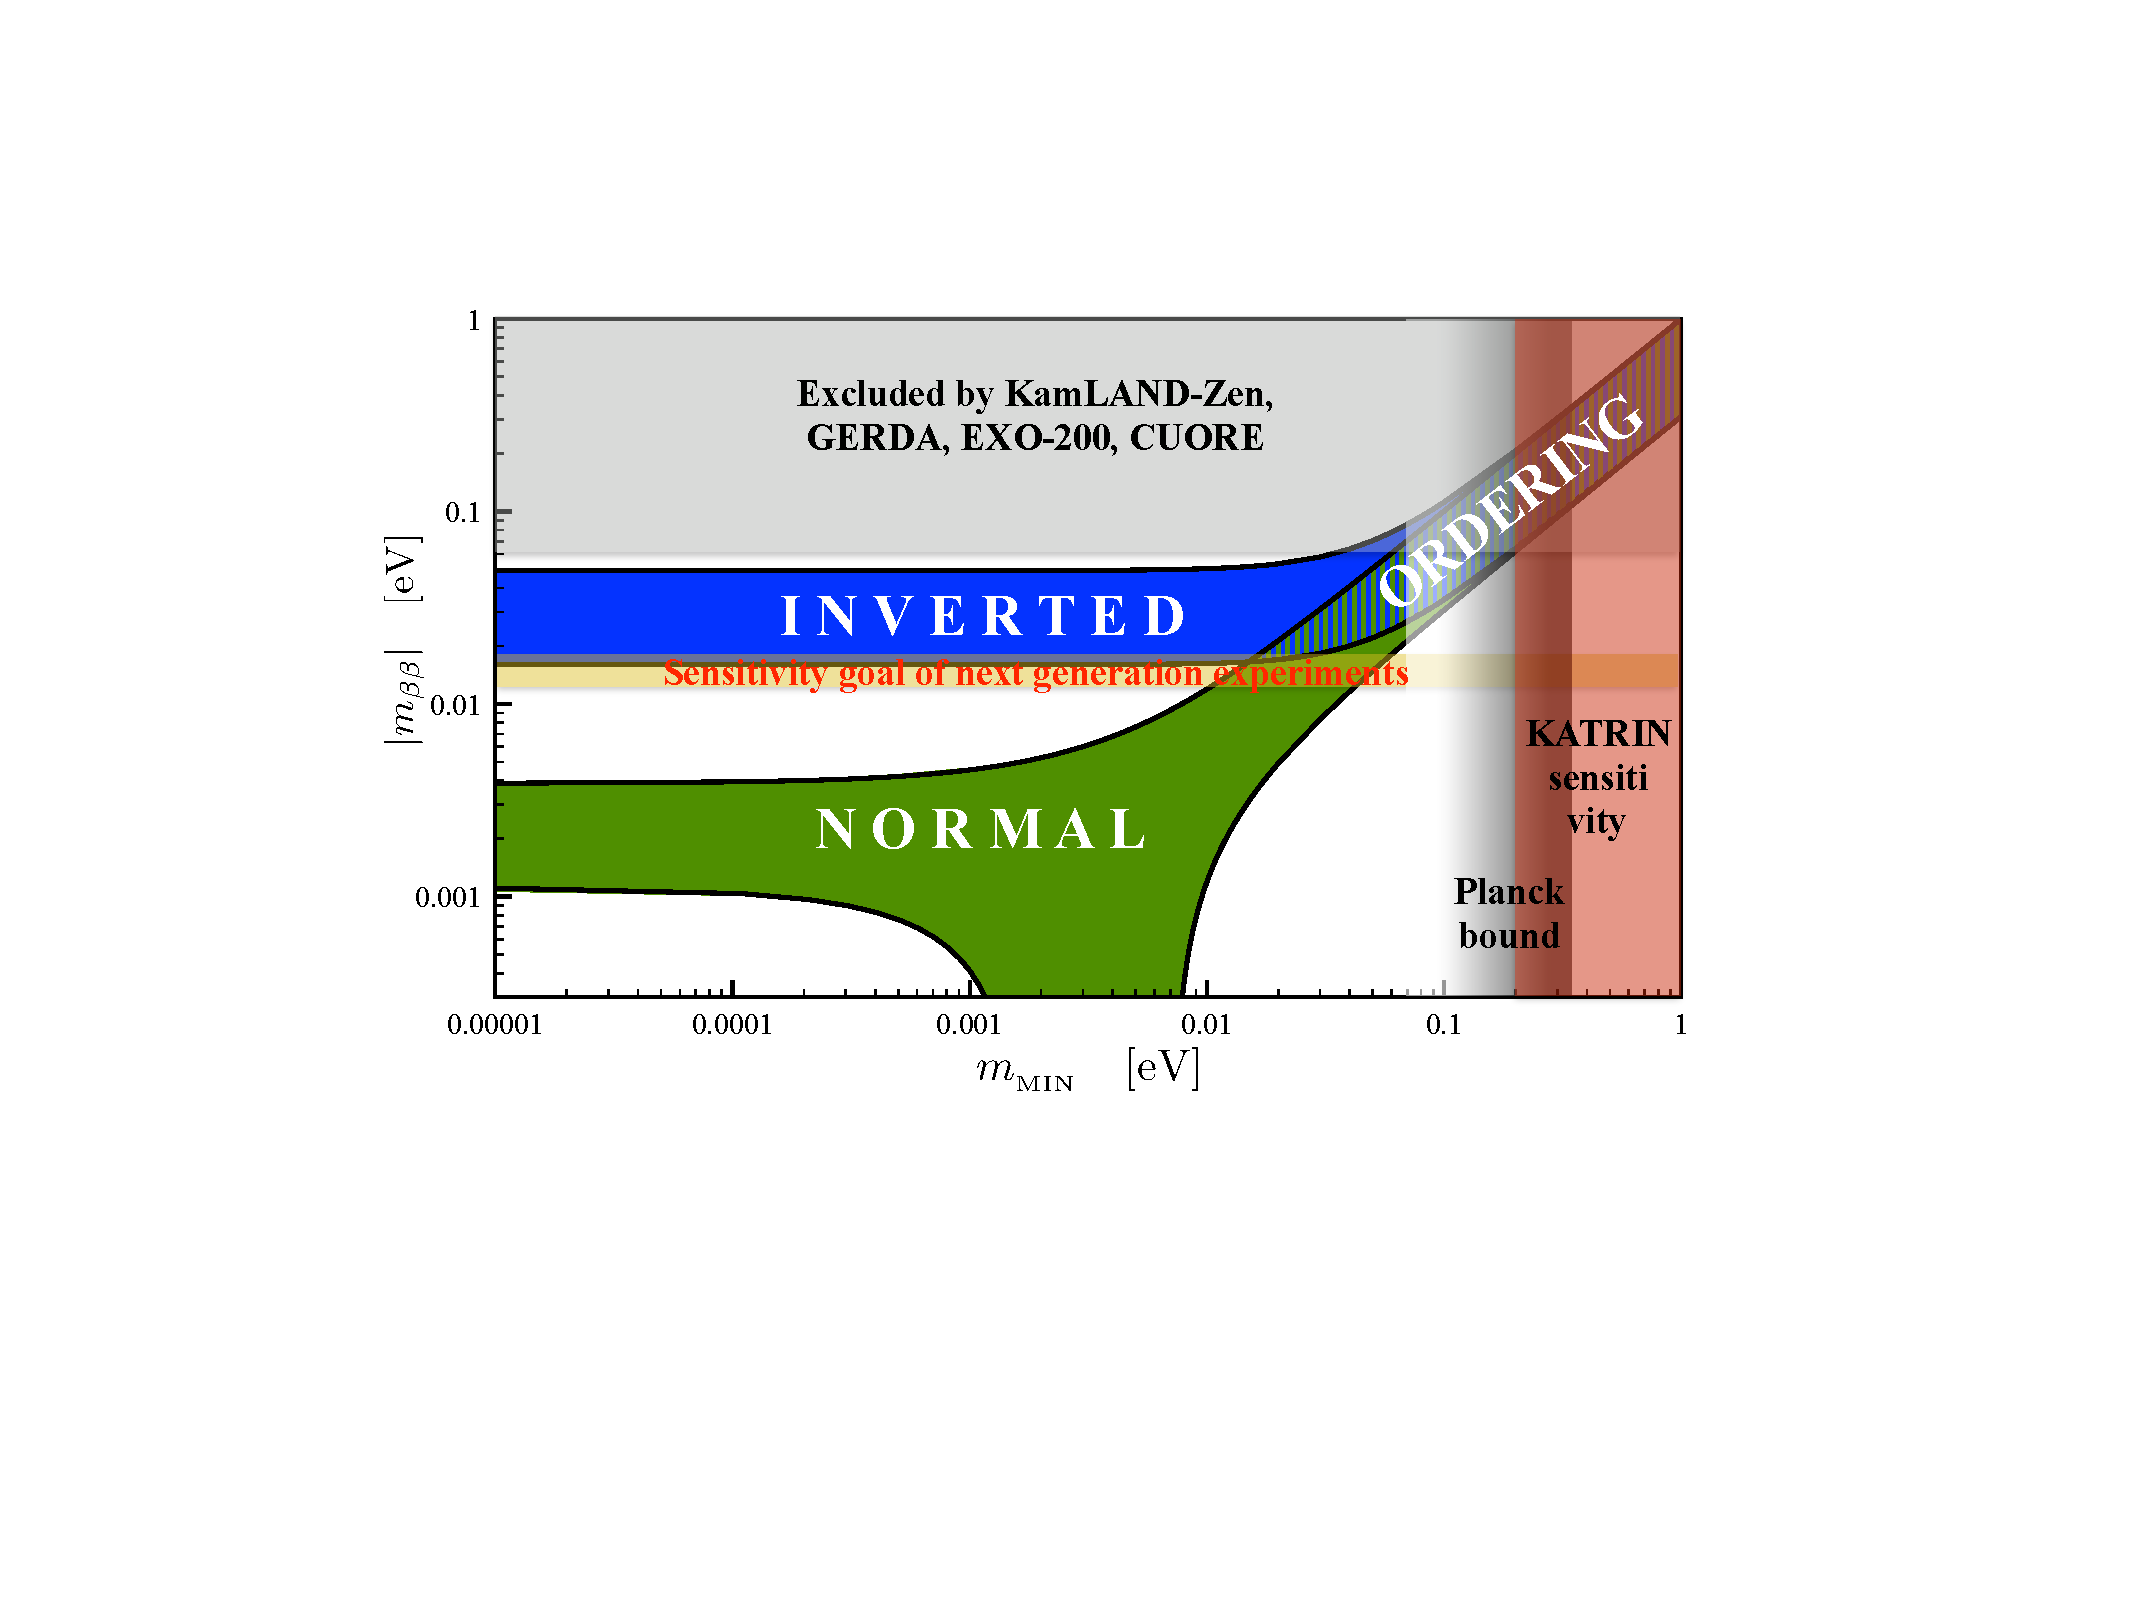
\includegraphics[width=0.8\textwidth]{img/APPECbetabetameff.pdf}
%\caption{\small The effective neutrino mass \mbb\ as a function of the mass of the lightest neutrino $m_\mathrm{MIN}$. From \cite{Giuliani:2019uno}.}  
%\label{fig:Majorana-Landscape}
%\end{figure}

\indent

When \mbb\ is represented as a function of the lightest neutrino mass $m_\mathrm{MIN}$, where $m_\mathrm{MIN}=m_1$ ($m_\mathrm{MIN}=m_3$) for normal (inverted) ordering of neutrino masses, one obtains a ``Majorana landscape'' (Figure~\ref{fig:numass_ordering}, right panel), defining the space of opportunity for discovery.

\indent

The so-called ``degenerate neutrino mass region'' portion of this landscape, defined by $m_1\simeq m_2\simeq m_3$ and reaching down to $\mbb \simeq \SI{50}{\meV}$, is being explored by the current generation of \bbonu\ experiments, achieving exposures in the range of hundred kilogram~year. 
%Five of these experiments (GERDA Phase II~\cite{GERDA:2020xhi}, MAJORANA DEMONSTRATOR~\cite{Majorana:2019nbd}, EXO-200~\cite{EXO-200:2019rkq}, KamLAND-Zen 400~\cite{KamLAND-Zen:2016pfg} and CUORE~\cite{CUORE:2021gpk}) have recently published the results of their analyses, extending the sensitivity of previous searches by more than one order of magnitude.  
The best limits on the half-life of a \bbonu\ isotope were obtained by KamLAND-Zen 400~\cite{KamLAND-Zen:2016pfg} in \Xe{136} ($\Tonu > \KZenTz$ at 90\% CL) and by GERDA Phase II~\cite{GERDA:2020xhi} in \Ge{76} ($\Tonu > \GerdaTz$ at 90\% CL). These half-life lower limits translate into a sensitivity to the effective neutrino mass of \KZenMbb\ and \GerdaMbb, respectively. 

\indent

The \Next\ experiment can reach a sensitivity to \Tonu\ similar to that achieved by  KamLAND-Zen ~\cite{Martin-Albo:2015rhw}, but with a very different systematic error. KamLAND-Zen boasts the largest exposure achieved so far by any \bbonu\ experiment (in excess of one ton$\cdot$year), but also the largest background rate, which needs to be subtracted from the data to search for a putative signal. Instead, \Next\ is expected to be near background-free at the 100 kg scale, and thus can provide a measurement wit very small uncertainty associated to background subtraction. 
 
The next step for the field is to fully explore the IH region. As shown in the right panel of Figure~\ref{fig:numass_ordering}, the light Majorana neutrino exchange mechanism combined with an inverted ordering of masses and $m_\mathrm{MIN}=m_3\simeq 0$ is expected to yield effective Majorana masses in the range \mbb = \SIrange{15}{50}{\meV}. Given the quadratic dependence of \mbb\ on the inverse half-life, see Eq.~\ref{eq:halflife}, increasing the sensitivity to \mbb\ by a factor of 4--10 (to some \SI{15}{\meV}) requires building experiments with a sensitivity to \Tonu\ between \IHTzl \; and  \IHTz \;  (depending on the value of the NME). This implies that the next generation of experiments sailing to fully explore the IH region will require a growth in exposure of 1--2 orders of magnitude.  Yet this alone is not sufficient, since the sensitivity to \Tonu\ grows linearly with exposure $Mt$, implying that the sensitivity for \mbb\ grows with $\sqrt{Mt}$, only for background-free experiments; instead, in a background-dominated regime, the sensitivity improves only with $\sqrt[4]{Mt}$.

%\begin{figure}[hb!]
%\centering
%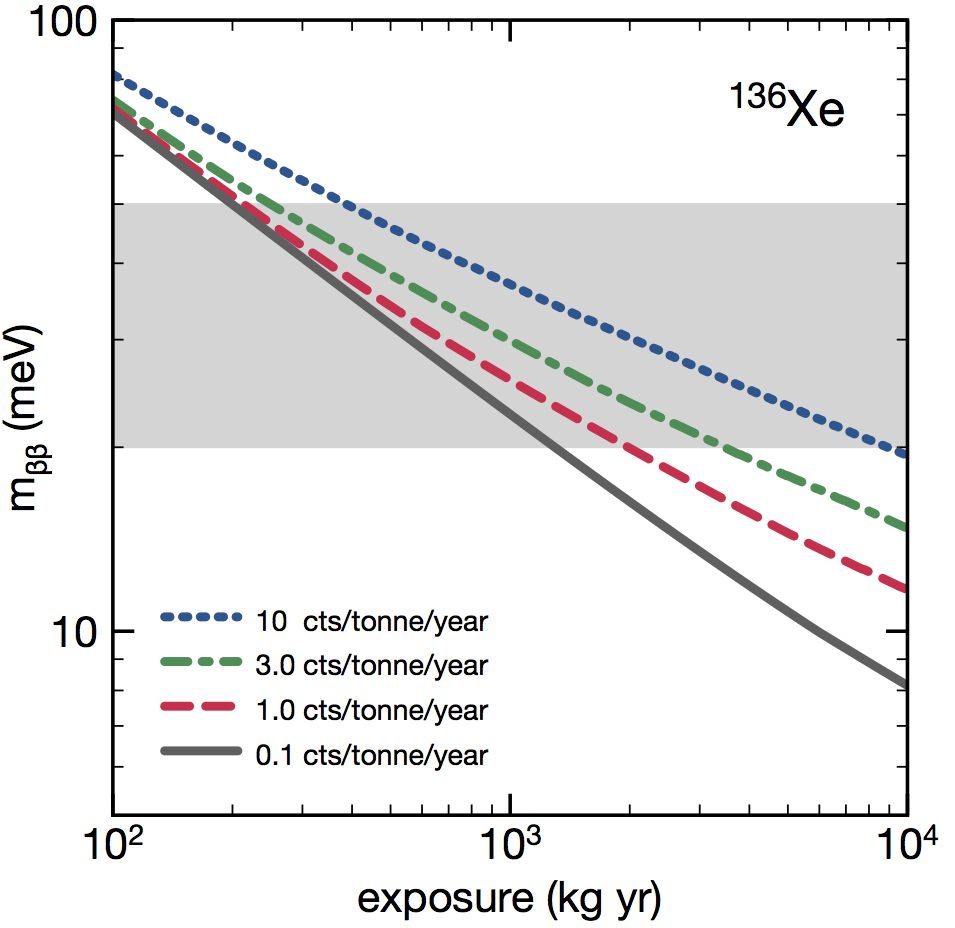
\includegraphics[width=0.4\textwidth]{img/sensi-xenon.png}
%\caption{\small Sensitivity of a fully efficient \XE\ experiment as a function of the exposure, for different background rates. From \cite{Martin-Albo:2015dza}.}
%\label{fig.Xe}
%\end{figure}
%
%The detrimental effect of the presence of background in next-generation experiments is illustrated by Figure~\ref{fig.Xe}, which shows the sensitivity to \mbb\ (using the IBM-2 NME \cite{Barea:2013bz}) of a fully efficient \XE\ experiment as a function of exposure, for different background rates.  An effective exposure of almost \SI{2}{\tonne\yr} is required for a full exploration of the IH region {\em in the background-free case}, \eg, for \BackgroundFreeLimit\ of background or less. The effective exposure increases to \SI{3}{\tonne\yr} for \AlmostBackgroundFreeLimit\ of background and degrades rapidly for larger backgrounds.  Thus, the conclusion is that the next generation of \bbonu\ experiments must feature target masses in the ton-range, while keeping the total background contained within \AlmostBackgroundFreeRequirement. 

\indent

%Beyond the next-generation step, the even more challenging priorities of the field will be determined by whether a \bbonu\ signal will be found by the first ton-scale experiments. If a \bbonu\ signal is found, the priority will be establishing which mechanism is responsible for the decay. 
%Information on the underlying mechanism can be potentially inferred from three experimental pieces of information: i) \bbonu\ half-life ratios between different isotopes, ii) \bbonu\ half-life ratios between different transitions to ground and excited states within the same isotope, and iii) single electron energy spectrum and angular distribution of the electrons for \bbonu\ candidate events.
 %If no \bbonu\ signal is found for \mbb $\gtrsim$ \SI{15}{\meV}, the priority will be extending the search to lower \mbb\ values and the next milestone would be covering the \mbb\ range predicted by NH and $m_\mathrm{MIN}=m_1\simeq 0$, that is \mbb = \SIrange{1}{4}{\meV}, see the right panel of Fig.~\ref{fig:numass_ordering}. This mass range translates into a sensitivity to \Tonu\  in the range \NHTl\ to \NHTz. 

\indent

Planning for the future (next-generation and beyond) \bbonu\ experiments is ongoing worldwide. In Europe, the recently released Double Beta Decay APPEC Committee
Report \cite{Giuliani:2019uno} recommended a multi-isotope program exploiting different technologies at the highest level of sensitivity to be supported, in order to mitigate the risks and to extend the physics reach of a possible discovery. The same report identifies LEGEND-1000 (\Ge{76}), CUPID (\Mo{100}) and NEXT-HD (\Xe{136}) as the most prominent next-generation projects with a strong European component. 
%In the US, a double beta decay Portfolio Review by DOE and the Snowmass particle physics community planning exercise are currently taking place. The US-DOE review focuses on LEGEND-1000 (\Ge{76}), nEXO (\Xe{136}) and CUPID (\Mo{100}) as main next-generation projects. The DOE portfolio also includes support, and motivation to pursue, future-looking programs beyond the next generation, including NEXT. 